%%
%% This is file `sample-sigchi-a.tex',
%% generated with the docstrip utility.
%%
%% The original source files were:
%%
%% samples.dtx  (with options: `sigchi-a')
%% 
%% IMPORTANT NOTICE:
%% 
%% For the copyright see the source file.
%% 
%% Any modified versions of this file must be renamed
%% with new filenames distinct from sample-sigchi-a.tex.
%% 
%% For distribution of the original source see the terms
%% for copying and modification in the file samples.dtx.
%% 
%% This generated file may be distributed as long as the
%% original source files, as listed above, are part of the
%% same distribution. (The sources need not necessarily be
%% in the same archive or directory.)
%%
%% The first command in your LaTeX source must be the \documentclass command.
\documentclass[sigchi-a]{acmart}

%%
%% \BibTeX command to typeset BibTeX logo in the docs
\AtBeginDocument{%
  \providecommand\BibTeX{{%
    \normalfont B\kern-0.5em{\scshape i\kern-0.25em b}\kern-0.8em\TeX}}}

%% Rights management information.  This information is sent to you
%% when you complete the rights form.  These commands have SAMPLE
%% values in them; it is your responsibility as an author to replace
%% the commands and values with those provided to you when you
%% complete the rights form.
% \setcopyright{acmcopyright}
% \copyrightyear{2019}
% \acmYear{2019}
% \acmDOI{10.1145/1122445.1122456}

%% These commands are for a PROCEEDINGS abstract or paper.
% \acmConference[Woodstock '18]{Woodstock '18: ACM Symposium on Neural
%   Gaze Detection}{June 03--05, 2018}{Woodstock, NY}
% \acmBooktitle{Woodstock '18: ACM Symposium on Neural Gaze Detection,
%   June 03--05, 2018, Woodstock, NY}
% \acmPrice{15.00}
% \acmISBN{978-1-4503-9999-9/18/06}


%%
%% Submission ID.
%% Use this when submitting an article to a sponsored event. You'll
%% receive a unique submission ID from the organizers
%% of the event, and this ID should be used as the parameter to this command.
%%\acmSubmissionID{123-A56-BU3}

%%
%% The majority of ACM publications use numbered citations and
%% references.  The command \citestyle{authoryear} switches to the
%% "author year" style.
%%
%% If you are preparing content for an event
%% sponsored by ACM SIGGRAPH, you must use the "author year" style of
%% citations and references.
%% Uncommenting
%% the next command will enable that style.
%%\citestyle{acmauthoryear}

%%
%% end of the preamble, start of the body of the document source.
\begin{document}

%%
%% The "title" command has an optional parameter,
%% allowing the author to define a "short title" to be used in page headers.
\title{Eye Tracking 2019 Project Report Group 7}

%%
%% The "author" command and its associated commands are used to define
%% the authors and their affiliations.
%% Of note is the shared affiliation of the first two authors, and the
%% "authornote" and "authornotemark" commands
%% used to denote shared contribution to the research.
\author{Viet Ta}
\affiliation{\institution{University of Eastern Finland}}
\email{taqu@uef.fi}

\author{Tuyet Tran}
\affiliation{\institution{University of Eastern Finland}}
\email{tuyet@uef.fi}

%%
%% By default, the full list of authors will be used in the page
%% headers. Often, this list is too long, and will overlap
%% other information printed in the page headers. This command allows
%% the author to define a more concise list
%% of authors' names for this purpose.
\renewcommand{\shortauthors}{Viet and Tuyet, et al.}

%%
%% The abstract is a short summary of the work to be presented in the
%% article.
\begin{abstract}
In this project, an algorithm called Identification by Dispersion Threshold is employed to identify fixations from raw gaze (x, y) locations recorded in time from subjects that shown images, which are recognized or unrecognized by observers. Subsequently, the fixation-identification's result will be analyzed and visualized. 
\end{abstract}

%%
%% The code below is generated by the tool at http://dl.acm.org/ccs.cfm.
%% Please copy and paste the code instead of the example below.
%%
% \begin{CCSXML}
% <ccs2012>
% <concept>
% <concept_id>10003120.10003121</concept_id>
% <concept_desc>Human-centered computing~Human computer interaction (HCI)</concept_desc>
% <concept_significance>500</concept_significance>
% </concept>
% <concept>
% <concept_id>10003120.10003121.10003122.10011749</concept_id>
% <concept_desc>Human-centered computing~Laboratory experiments</concept_desc>
% <concept_significance>500</concept_significance>
% </concept>
% </ccs2012>
% \end{CCSXML}

% \ccsdesc[500]{Human-centered computing~Human computer interaction (HCI)}
% \ccsdesc[500]{Human-centered computing~Laboratory experiments}

%%
%% Keywords. The author(s) should pick words that accurately describe
%% the work being presented. Separate the keywords with commas.
\keywords{eye-tracking, fixation, saccade, mfd, msa}


%%
%% This command processes the author and affiliation and title
%% information and builds the first part of the formatted document.
\maketitle


\section{Algorithm}
\subsection{Identification by Dispersion Threshold (I-DT)}

I-DT is mostly used for low-speed data (50Hz).
It can detect (only) \textbf{fixation} by finding \textbf{data samples} that \textbf{close enough to one another} for a \textbf{specified minimal period of time}.

Beside from raw data samples, it requires 2 input parameters, which are duration-threshold and dispersion-threshold, to able to detect fixations.
For example, if the duration-threshold is 100ms and dispersion-threshold is 1-degree, then data samples that stay within 1-degree diameter for at least 100ms is \textbf{fixation}. \cite{Holmqvist11}

I-DT algorithm uses a moving window to detect fixations in order of sequence of sample data points.
Initially, within the input duration-threshold, the moving window spans over first points of data samples. Next, dispersion of points will be calculated as the summing differences between maximum and minimum value of window points' x and y.
\begin{equation}
D = max(x)-min(x)+max(y)-min(y)
\end{equation}
\begin{itemize}
\item Now, if dispersion is above dispersion-threshold, move window 1 point to the right within data samples.
\item In contrast, if dispersion is below dispersion-threshold, then the window is promisingly a fixation. In this case, the window will be expanded to the right (add more points) until dispersion is above threshold; the centroid of this new window points is registered as a fixation and these window points be removed from data samples.
\end{itemize}
The process continues until moving window reaches the end point of data samples. All detected fixations be returned. \cite{Punde16} 


\subsection{Setting of I-DT Algorithm}
As mentioned in previous section, I-DT requires 2 pre-set parameters, which are \textbf{duration threshold} and \textbf{dispersion threshold}. Regarding the task of detect fixations, our group used 2 distinct settings for I-DT Algorithm.
\begin{itemize}
    \item \textsc{setting1}: $dispersion-threshold = 1$ (degree), $duration-threshold = 0.1$ (s).
    \item \textsc{setting2}: $dispersion-threshold = 2$ (degrees), $duration-threshold = 0.1$ (s).
\end{itemize}

\subsubsection{Selected Setting for The Processing of Further Tasks}
After comparing the fixation-detection results, we chose output from \textsc{setting1} for further tasks processing as it seems to support a more accurate fixation-detection.

\subsection{I-DT Pseudo Code \cite{Salvucci2000}}
\textit{Input: data (data of each row), dispersion-threshold, window-size and sampling-frequency (to compute fixation time)}


WHILE there are still point in data

o Initialize window over first points within (initial) window-size and calculate window's dispersion

o IF dispersion of window points <= dispersion-threshold
\begin{itemize}
    \item Add additional points to the window until dispersion > dispersion-threshold
    \item Note a fixation at the centroid of window points
    \item Note fixation time
    \item Remove window points from raw data
\end{itemize}
    
o ELSE 
\begin{itemize}
    \item Remove first point from window
\end{itemize}


RETURN centroid of fixations and their fixation time


\textit{See \url{https://github.com/envil/eye-tracking-2019/blob/master/project/src/idt.py}}   

\begin{marginfigure}
  
\end{marginfigure}

\subsection{Calculating of MFA and MSA}
\subsubsection{MFA}
It's quite straightforward to calculate MFA:

\begin{equation}
    MFA = FixationEndTime - FixationStartTime
\end{equation} 
\subsubsection{MSA} Firstly we need to calculate the Euclidean distance between two fixation. Based on the experiment set up (display size: $195\times113mm$, distance to screen $450mm$, resolution $1400\times1400$), we can calculate the unit size. From there we can calculate the Euclidean distance between two fixations.

Then, we convert the distance to angle:
\begin{equation}
    angle=2\times \arctan\left(\frac{distance}{2\times DistanceToScreen}\right)
\end{equation}
% \subsection{Detect fixation, Return Fixation Time and Centroid Point of Fixation (task1)}
% FOR each row in \textbf{train.csv} file

% FOR each row that have the first value equal to 's7' or 's17' or 's27' or 's3' or 's13' or 's23'
% \begin{itemize}
% \item Save \textbf{sid} and \textbf{known} to an array
% \item Convert x and y values to float and save to another array with format of point (x, y)

% (These points array will be inputted to a \textit{detect fixations function}.)
% \end{itemize}   
% \textit{See \url{https://github.com/envil/eye-tracking-2019/blob/master/project/src/main.py}}    

% \subsection{Data Analyzing (task2)}
% Details step for task 2... (pseudo code, link to source code)

% \subsection{Report Analyzed Data in Details (task3)}
% Details step for task 3... (pseudo code, link to source code)

% \subsection{Plot Analyzed Data (task4)}
% Details step for task 4... (pseudo code, link to source code)


\section{Data Analyzing Results}
The analyzed data includes \textbf{mean fixation durations}, \textbf{mean saccade amplitudes } and their \textbf{standard deviation} for each subject as well as all subjects (\textbf{recognized} and \textbf{unregconized}) is reported in Task 2's Ouput Table \textbf{\ref{table:outputTask2}}.

\begin{table}[]
    \centering
    \caption{Task 2's Output}
    \label{table:outputTask2}
    \begin{tabular}{1|2|3|4|5|6}
      \textbf{sid} &\textbf{known} &\textbf{mfd} &\textbf{mfd-sd} &\textbf{msa} &\textbf{msa-sd}\\
      \hline
      s7 &True &0.22 &0.08 &6.44 &4.45\\ 
      s7 &False &0.21 &0.10 &5.94 &4.69\\  
      s17 &True &0.21 &0.11 &6.62 &4.58\\ 
      s17 &False &0.21 &0.10 &6.14 &4.27\\  
      s27 &True &0.18 &0.08 &6.63 &4.32\\ 
      s27 &False &0.18 &0.08 &6.91 &5.21\\ 
      s3 &True &0.20 &0.12 &6.69 &5.54\\ 
      s3 &False &0.18 &0.08 &6.18 &4.81\\ 
      s13 &True &0.28 &0.27 &4.71 &4.63\\ 
      s13 &False &0.24 &0.23 &5.60 &5.09\\ 
      s23 &True &0.18 &0.07 &3.95 &4.09\\ 
      s23 &False &0.22 &0.12 &4.61 &4.94\\ 
      all &True &0.21 &0.13 &6.16 &4.70\\ 
      all &False &0.21 &0.15 &5.99 &4.95\\ 
    \end{tabular}
\end{table}

The details report for analyzed data following Task 3's requirements can be found here \textbf{\url{https://github.com/envil/eye-tracking-2019/blob/master/project/src/output/group7.csv}}

The plots for analyzed data following Task 4's requirements can be found here \textbf{\url{https://github.com/envil/eye-tracking-2019/tree/master/project/src/figures/stats}}


\section{Discussion of Results}
From the analyzed results, we deduced that there is no significant differences between \textbf{MFD} of \textbf{recognized} and \textbf{unrecognized} subjects. However, the \textbf{recognized subjects' SD} is higher than the \textbf{unrecognized ones}. 

The deduced statements can be explained by following hypothesis:
\begin{itemize}
    \item When an observer recognizes a subject, he or she tends to pay longer attention to some particular fixations, hence SD between recognized subject's fixations is higher.
    \item On the contrary, when an observer cannot recognize a subject, he (she) will unconsciously move his (her) sight between points faster (saccade). Meaning that there is less points being observed longer than the others, therefore, SD of the subject is lower.
\end{itemize}

Regarding to the MSA, we noticed that the \textbf{mean} and \textbf{SD} of \textbf{regconized subjects} are \textbf{greater} than \textbf{unregconized ones}. This can be reasoned by following assumption:
\begin{itemize}
    \item When an observer cannot recognize a subject, he (she) has no particular sight' target. Hence the saccades' velocity will be slower and less-varying.  
    \item Contrarily, when an observer recognize a subject, he (she) will observe based on points in his (her) memory. Having kwown the points beforehand, the saccades's velocity of observer will be higher and more-varying.
\end{itemize}


\section{Contribution of Group Members}
\begin{itemize}
    \item Tuyet Tran (299856): 40\%
    \item Viet Ta (299954): 60\%
    \item Eetu Mynttinen (299464): 0\%
\end{itemize}



% Again, in either environment, you can use any of the symbols and
% structures available in \LaTeX\@; this section will just give a couple
% of examples of display equations in context.  First, consider the
% equation, shown as an inline equation above:
% \begin{equation}
%   \lim_{n\rightarrow \infty}x=0
% \end{equation}
% Notice how it is formatted somewhat differently in
% the \textbf{displaymath}
% environment.  Now, we'll enter an unnumbered equation:
% \begin{displaymath}
%   \sum_{i=0}^{\infty} x + 1
% \end{displaymath}
% and follow it with another numbered equation:
% \begin{equation}
%   \sum_{i=0}^{\infty}x_i=\int_{0}^{\pi+2} f
% \end{equation}
% just to demonstrate \LaTeX's able handling of numbering.

% \section{Figures}

% The ``\verb|figure|'' environment should be used for figures. One or
% more images can be placed within a figure. If your figure contains
% third-party material, you must clearly identify it as such, as shown
% in the example below.
% \begin{marginfigure}
%   \centering
%   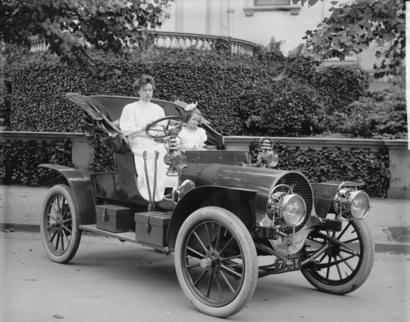
\includegraphics[width=\linewidth]{sample-franklin}
%   \caption{1907 Franklin Model D roadster. Photograph by Harris \&
%     Ewing, Inc. [Public domain], via Wikimedia
%     Commons. (\url{https://goo.gl/VLCRBB}).}
%   \Description{The 1907 Franklin Model D roadster.}
% \end{marginfigure}


%%
%% The next two lines define the bibliography style to be used, and
%% the bibliography file.
\bibliographystyle{ACM-Reference-Format}
\bibliography{sample-base}

%%
%% If your work has an appendix, this is the place to put it.
\appendix

\end{document}
\endinput
